%-----------------------------------------------------------------------
%
%   UFRJ  - Universidade Federal do Rio de Janeiro
%   COPPE - Coordena��o dos Programas de P�s-gradua��o em Engenharia
%   PEE   - Programa de Engenharia El�trica
%
%   COE-835  Controle adaptativo
%
%   Relat�rio da simula��o
%                                                         Ramon R. Costa
%                                                         05/out/09, Rio
%-----------------------------------------------------------------------
\documentclass[11pt,a4paper]{article}
\usepackage[latin1]{inputenc} %pacote para utilizar palavras acentuadas
\usepackage{amsmath,amssymb}  %pacotes do AMS
\usepackage{latexsym}         %pacote para incluir s�mbolos (ex.\Box)
\usepackage{fancybox,fancyhdr}%pacote com frescuras
\usepackage{graphicx}         %pacote para incluir figuras tipo eps
\usepackage[portuguese]{babel}
\usepackage{xcolor}
\usepackage{float} 
\usepackage{epstopdf}
\usepackage[inline]{enumitem}
\usepackage[a4paper]{hyperref}% Make sure it comes last of your loaded packages
\hypersetup{
  verbose,
  plainpages=false,
  bookmarks=true,
  colorlinks=true,
  linkcolor=blue
}
     
%----------------------------------------------------------------------
%
%   Macros utilizados no LATEX
%                                                       Ramon R. Costa
%                                                       13/out/17, Rio
%----------------------------------------------------------------------
\newcount\m
\newcount\n

\def\twodigits#1{\ifnum #1<10 0\fi \number#1}

\def\hours{\n=\time \divide\n 60
    \m=-\n \multiply\m 60 \advance\m \time
    \twodigits\n:\twodigits\m}

\def\hora{\hours}

\def\fim{
  \medskip
  \begin{center}
    \rule[1mm]{30mm}{0.14mm}$\diamond$\rule[1mm]{30mm}{0.14mm}
  \end{center}
}

%----------------------------------------------------------------------
% A4 paper size & margins
\setlength {\textheight}    {25cm}%
\setlength {\textwidth}     {17.5cm}%
\setlength {\parindent}     {0mm}%
\setlength {\parskip}       {1mm}%
\setlength {\topmargin}     {-14mm}%
\setlength {\oddsidemargin} {-6mm}%
\setlength {\evensidemargin}{-6mm}%
\setlength {\columnsep}     {6mm}%

%----------------------------------------------------------------------
\def\codigo{COE-835}
\def\disciplina{Controle adaptativo}
\def\periodo{3o. período/2017}
\def\professor{Ramon}

\newcommand{\BOX}[1]{
  \framebox{{\color{magenta}\rule[-3mm]{1mm}{9mm}} ~~$\displaystyle
  \begin{aligned} #1 \end{aligned}$~~}\pagestyle{plain}
}

\newcommand{\RED}[1]{\colorbox{white}{\textcolor{red}{#1}}}
%\newcommand{\WoR}[1]{\colorbox{red}{\textcolor{white}{#1}}}
\newcommand{\BLU}[1]{\colorbox{white}{\textcolor{blue}{#1}}}
\newcommand{\GRE}[1]{\colorbox{green}{\textcolor{black}{#1}}}
\newcommand{\HI}[1]{\colorbox{yellow}{\textcolor{black}{#1}}}  %% Highlithed text

\newcommand{\estrela}[1]{
  \def\TXT{\RED{$\bigstar$ }}
  \hspace*{5mm}\TXT \hfill
  \parbox[t]{ \textwidth - \widthof{\TXT} - 5mm}{#1}
  \par
}

\def\Ltwo{\mbox{${\mathcal L}_2$}}
\def\Linf{\mbox{${\mathcal L}_\infty$}}

\newcommand{\sign}{\mbox{sign}}

\newcommand{\equacao}[2]{
  \makebox[40mm][l]{#1 \dotfill}: \quad \parbox[t]{8cm}
	{\begin{equation} \displaystyle
  \begin{aligned}
    #2
  \end{aligned} \end{equation}} \\
}

\newcommand{\sref}[1]{Section~\ref{#1}}
\newcommand{\fref}[1]{Fig.~\ref{#1}}
\newcommand{\tref}[1]{Table~\ref{#1}}
\newcommand{\thref}[1]{Theorem~\ref{#1}}
\newcommand{\aref}[1]{Assumption~\ref{#1}}
\newcommand{\norm}[1]{\left\lVert#1\right\rVert}
%\renewcommand{\qedsymbol}{}
\newcommand{\rev}[1]{{\color{red}#1}}
%\newcommand{\mat}[1]{\begin{bmatrix}#1\end{bmatrix}}

\newtheorem{remark}{Remark}
\newtheorem{lemma}{Lema}

%----------------------------------------------------------------------


\begin{document}
%---------------------------------------------------------------------
\pagestyle{fancy}%
\renewcommand{\headrulewidth}  {0.4pt}%
\renewcommand{\footrulewidth}  {0.4pt}%
\lhead{\bfseries{Relat�rio do Trabalho 2}}%
\chead{}%
\rhead{\bfseries\thepage}%
\lfoot{}%
\cfoot{}%
\rfoot{[\hours] \quad \today}%
%---------------------------------------------------------------------
\begin{center}
  \huge{COE-835  Controle  adaptativo}  \\[20mm]

  \Large{Simula��es do Trabalho 2} \\[20mm]
\end{center}

\textbf{Grupo:} \quad \parbox[t]{10cm}{
Guilherme Pires Sales de Carvalho \\[2mm]
Matheus Ferreira dos Reis \\[2mm]
Renan Salles de Freitas \\[10mm]
}

\textbf{Algoritmo:} \quad \HI{MRAC Indireto}\\[2mm]

\bigskip%
Caso: \quad \parbox[t]{10cm}{
  $~n = 1$ \quad (ordem da planta) \\[2mm]
  $n^* = 1$ \quad (grau relativo) \\[2mm]
  $n_p = 1$ \quad (\# de par�metros) \\[15mm]
}

%---------------------------------------------------------------------
\tableofcontents
\newpage
%---------------------------------------------------------------------
%---------------------------------------------------------------------
\section{Resumo das equa��es do m�todo}

Abaixo, resumimos algumas das principais equa��es utilizadas no m�todo.

\vspace{20mm}

 \newpage
\input{MRAC_indireto}
%---------------------------------------------------------------------
\section{Diagramas de blocos}

 \newpage
%---------------------------------------------------------------------
\section{Resultados das simula��es}

%Simula��o utilizando \HI{\texttt{Matlab/Simulink}}.

Nas simula��es, procuramos avaliar o comportamento do sistema para as seguintes condi��es:
%
\begin{enumerate*}[label=(\roman*)]
\item condi��o inicial $\theta(0)$;
\item sinal de refer�ncia $r(t)$;
\item ganho de adapta��o $\gamma$.
\end{enumerate*}

Apresentaremos os resultados obtidos atrav�s de simula��es no ambiente \HI{\texttt{Matlab/Simulink}} e os discutiremos na pr�xima se��o.

\subsection{Simula��o \#1}

Inicialmente, desejamos verificar o comportamento do sistema para varia��es no
sinal de refer�ncia $r(t)$ para podermos analisar a influ�ncia da persist�ncia
de excita��o.

%\bigskip%
%Par�metros e condi��es iniciais :
%
\begin{align*}
  y &= \frac{1}{s+2}u\,,  &  \Lambda &= \frac{1}{s+1}\,, & \theta(0) &= 0\,, \\
  \gamma &= 5\,, & r &= \HI{1, $1+5\textrm{sin}(t)$}\, \,.
\end{align*}

\bigskip%
\begin{figure}[H]
  \centering
  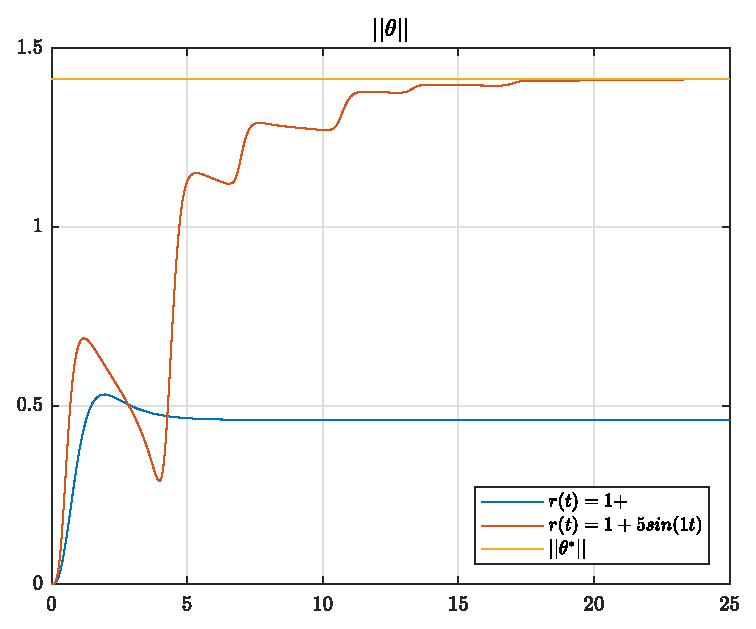
\includegraphics[width=12cm]{figs/gradiente/modtheta/sim01_r1r2.eps} \\[2mm]
\end{figure}

\begin{figure}[H]
  \centering
  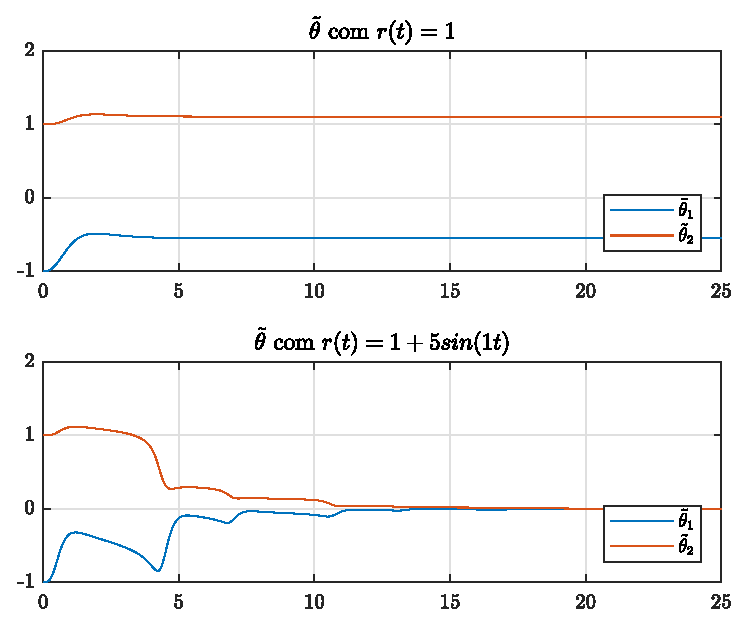
\includegraphics[width=12cm]{figs/gradiente/tiltheta/sim01_r1r2.eps} 
\end{figure}


\begin{figure}[H]
  \centering
  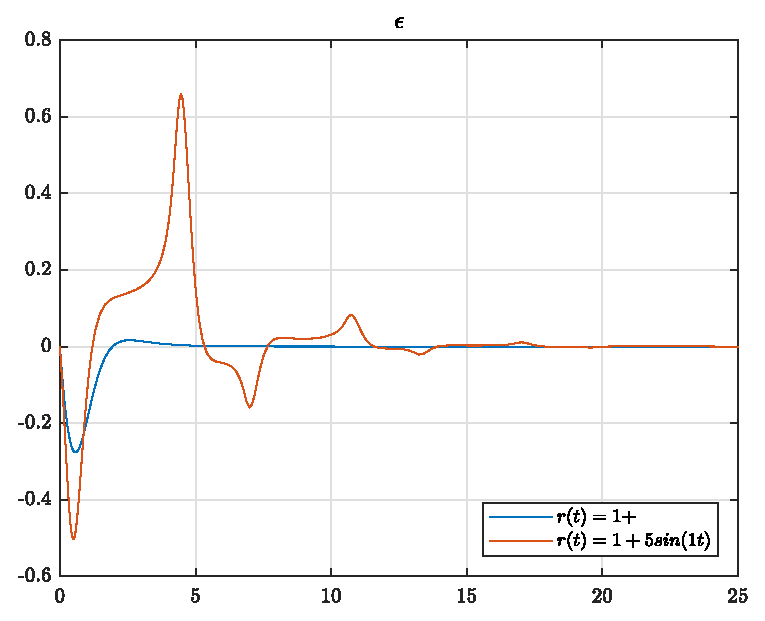
\includegraphics[width=12cm]{figs/gradiente/epsilon/sim01_r1r2.eps} 
\end{figure}

\newpage%

\begin{align*}
  y &= \frac{s+1}{s+4s+4}u\,,  &  \Lambda &= \frac{1}{s+2s+1}\,, & \theta(0) &=
  0\,,\\
  \gamma &= 10\,, & r &= \HI{$10\textrm{sin}(0.63493t)$} e
  \HI{$30\textrm{sin}(0.63493t)+25\textrm{sin}(4.5669t)$}\, \,.
\end{align*}

\bigskip%
\begin{figure}[H]
  \centering
  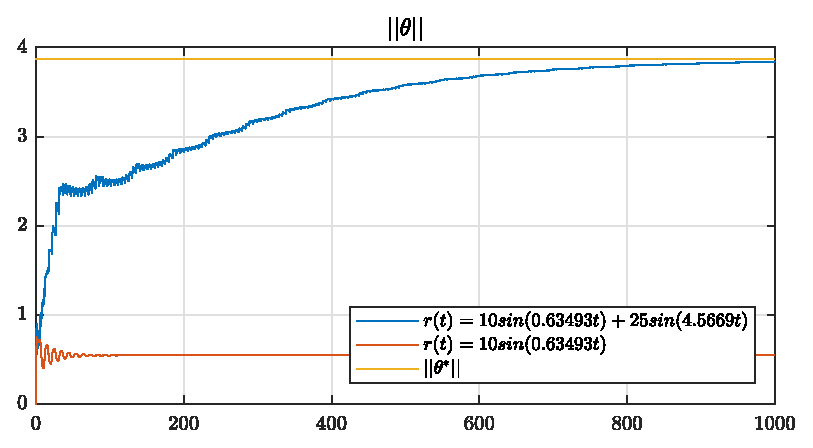
\includegraphics[width=12cm]{figs/gradiente/modtheta/sim02_r1r2.eps} \\[2mm]
\end{figure}

\begin{figure}[H]
  \centering
  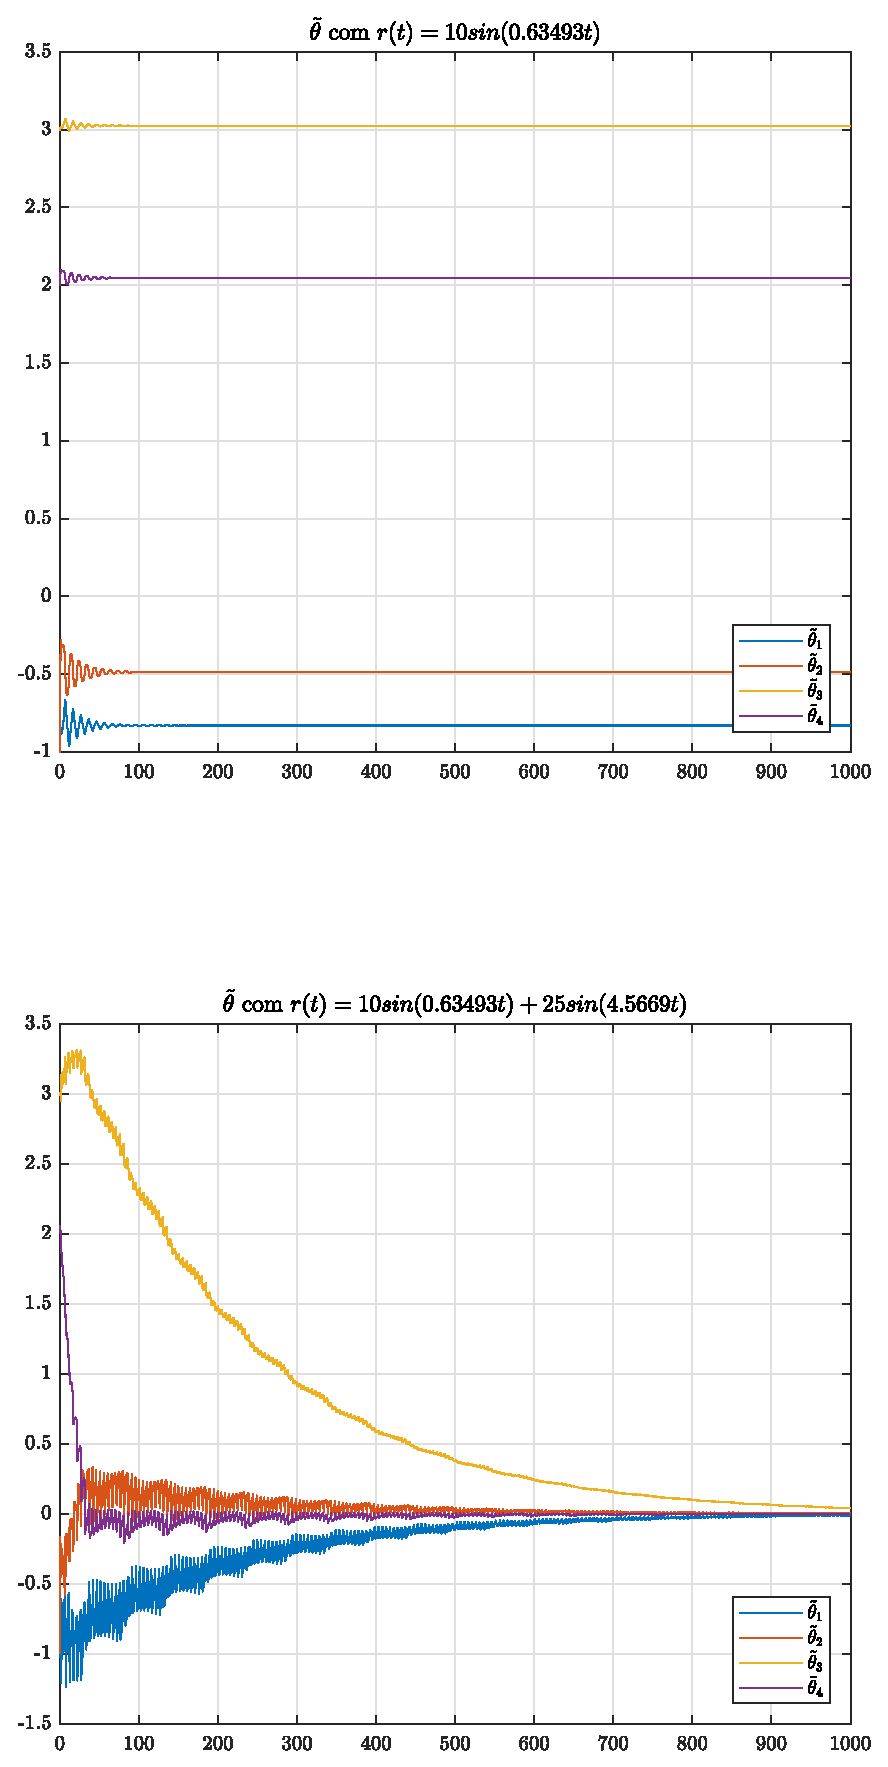
\includegraphics[width=12cm]{figs/gradiente/tiltheta/sim02_r1r2.eps} 
\end{figure}


\begin{figure}[H]
  \centering
  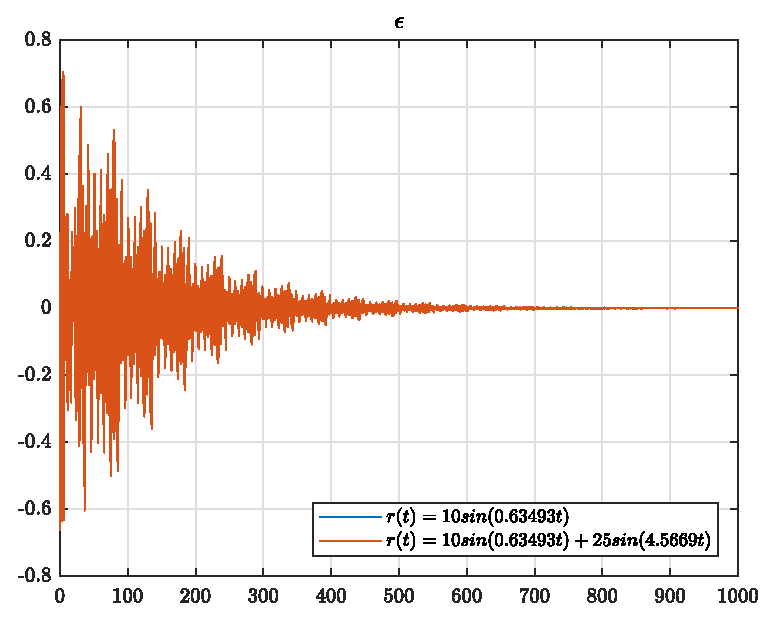
\includegraphics[width=12cm]{figs/gradiente/epsilon/sim02_r1r2.eps} 
\end{figure}
%---------------------------------------------------------------------
\subsection{Simula��o \#2}

Na segunda simula��o, observamos o comportamento do sistema para varia��es no p�lo do filtro.

%\bigskip%
%Par�metros e condi��es iniciais:
%
\begin{align*}
  a_p &= -2\,,  &  y_p(0) &= 0\,, & \theta(0) &= 0\,, \\
  a_m &= 1\,,   &  y_m(0) &= 0\,, & \gamma &= 5\,, \\
  r &= 1\,, & a_f &= \HI{3, 5}\,.
\end{align*}

\begin{figure}[H]
  \centering
  \includegraphics[width=12cm]{figs/e0/af3af5.eps} \\[2mm]
\end{figure}

\begin{figure}[H]
  \centering
  \includegraphics[width=12cm]{figs/epsilon/af3af5.eps} 
\end{figure}


\begin{figure}[H]
  \centering
  \includegraphics[width=12cm]{figs/theta/af3af5.eps} 
\end{figure}

\begin{figure}[H]
  \centering
  \includegraphics[width=12cm]{figs/yp/af3af5.eps} 
\end{figure}

\begin{figure}[H]
  \centering
  \includegraphics[width=12cm]{figs/u/af3af5.eps} 
\end{figure}

\newpage%
%---------------------------------------------------------------------
\subsection{Simula��o \#3}

Na terceira simula��o, observamos o comportamento do sistema para varia��es no p�lo desconhecido da planta.

%\bigskip%
%Par�metros e condi��es iniciais:
%
\begin{align*}
  a_p &= \HI{-2, -5}\,,  &  y_p(0) &= 0\,, & \theta(0) &= 0\,, \\
  a_m &= 1\,,   &  y_m(0) &= 0\,, & \gamma &= 5\,, \\
  r &= 1\,, & a_f &= 1\,.
\end{align*}

\begin{figure}[H]
  \centering
  \includegraphics[width=12cm]{figs/e0/ap-2ap-5.eps} \\[2mm]
\end{figure}

\begin{figure}[H]
  \centering
  \includegraphics[width=12cm]{figs/epsilon/ap-2ap-5.eps} 
\end{figure}


\begin{figure}[H]
  \centering
  \includegraphics[width=12cm]{figs/theta/ap-2ap-5.eps} 
\end{figure}

\begin{figure}[H]
  \centering
  \includegraphics[width=12cm]{figs/yp/ap-2ap-5.eps} 
\end{figure}

\begin{figure}[H]
  \centering
  \includegraphics[width=12cm]{figs/u/ap-2ap-5.eps} 
\end{figure}

\newpage%
%---------------------------------------------------------------------

\subsection{Simula��o \#4}

Na simula��o 4, variamos o p�lo do modelo de refer�ncia utilizado.

%\bigskip%
%Par�metros e condi��es iniciais:
%
\begin{align*}
  a_p &= -2\,,  &  y_p(0) &= 0\,, & \theta(0) &= 0\,, \\
  a_m &= \HI{2, 5}\,,   &  y_m(0) &= 0\,, & \gamma &= 5\,, \\
  r &= 1\,, & a_f &= 1\,.
\end{align*}

\begin{figure}[H]
  \centering
  \includegraphics[width=12cm]{figs/e0/am2am5.eps} \\[2mm]
\end{figure}

\begin{figure}[H]
  \centering
  \includegraphics[width=12cm]{figs/epsilon/am2am5.eps} 
\end{figure}


\begin{figure}[H]
  \centering
  \includegraphics[width=12cm]{figs/theta/am2am5.eps} 
\end{figure}

\begin{figure}[H]
  \centering
  \includegraphics[width=12cm]{figs/yp/am2am5.eps} 
\end{figure}

\begin{figure}[H]
  \centering
  \includegraphics[width=12cm]{figs/u/am2am5.eps} 
\end{figure}

\newpage%
%---------------------------------------------------------------------

\subsection{Simula��o \#5}

Por �ltimo, observamos o comportamento do sistema para varia��es nas condi��es iniciais da planta.

%\bigskip%
%Par�metros e condi��es iniciais:
%
\begin{align*}
  a_p &= -2\,,  &  y_p(0) &= \HI{0, 5}\,, & \theta(0) &= 0\,, \\
  a_m &= 1\,,   &  y_m(0) &= 0\,, & \gamma &= 5\,, \\
  r &= 1\,, & a_f &= 1\,.
\end{align*}

\begin{figure}[H]
  \centering
  \includegraphics[width=12cm]{figs/e0/yp00yp05.eps} \\[2mm]
\end{figure}

\begin{figure}[H]
  \centering
  \includegraphics[width=12cm]{figs/epsilon/yp00yp05.eps} 
\end{figure}


\begin{figure}[H]
  \centering
  \includegraphics[width=12cm]{figs/theta/yp00yp05.eps} 
\end{figure}

\begin{figure}[H]
  \centering
  \includegraphics[width=12cm]{figs/yp/yp00yp05.eps} 
\end{figure}

\begin{figure}[H]
  \centering
  \includegraphics[width=12cm]{figs/u/yp00yp05.eps} 
\end{figure}

\newpage%
%--------------------------------------------------------------------- \newpage
%---------------------------------------------------------------------
\section{Discuss�o}

A \textbf{simula��o \#1} mostra o comportamento do sistema para varia��es no sinal de refer�ncia. Como esperado e demonstrado na se��o 3.5 do livro \textit{Adaptive
Control Design and Analysis} de Gang Tao, a converg�ncia dos par�metros s� �
garantida quando o sinal de refer�ncia possui o mesmo n�mero de
frequ�ncias que o n�mero de par�metros desconhecidos (excita��es persistentes).

Na simula��o 1.1, o sistema � de primeira ordem com dois
par�metros desconhecidos. Logo, s�o necess�rias duas frequ�ncias diferentes no
sinal de refer�ncia para garantir que o erro de estima��o $\tilde{\theta}$
convirja para zero. Isso � verificado, j� que $\tilde{\theta}$ converge para
zero quando $r=1+5\textrm{sin}(t)$ (frequ�ncia em $\omega=0, \omega=1,
\omega=-1$) e n�o converge para zero quando o sinal possui apenas uma frequ�ncia
($r=1$). Um comportamento semelhante � verificado para os sistemas de segunda e
terceira ordens (simula��es 1.2 e 1.3, respectivamente). Vale observar que, em
todos os casos, $\epsilon = \tilde{\theta}^\intercal \phi$ converge para zero,
como � provado por Lyapunov.  Isso significa que, apesar de a estima��o dos
par�metros n�o ter garantia de converg�ncia para zero, os vetores $\tilde{\theta}$ e $\phi$ entram em quadratura, ou seja, ficam ortogonais.

A \textbf{simula��o \#2} mostra o comportamento do sistema para varia��es no
ganho de adapta��o $\Gamma$ para o m�todo do gradiente normalizado. Nesse caso, a varia��o da estima��o de par�metros � descrita pela f�rmula: $\dot{\theta}(t) = -\Gamma \, \phi(t) \, \epsilon(t) / m^2(t)$. Portanto, a varia��o � proporcional ao ganho de adapta��o, quanto maior o par�metro, mais r�pida ser� a estima��o. J� no caso do m�todo \textit{least-squares} normalizado, o valor inicial do ganho n�o impacta muito no regime transit�rio.

A \textbf{simula��o \#3} mostra o comportamento do sistema para varia��es nas condi��es iniciais. A rapidez da converg�ncia depende de qu�o pr�ximo os par�metros estimados est�o dos par�metros reais. Na simula��o 3.1, por exemplo, a converg�ncia � mais r�pida quando $\theta = \textbf{0}, \theta^* = \left[1 \, -1\right]$, por�m, na simula��o 3.3, ela � mais r�pida quando $\theta = \textbf{1}$, pois $\theta^* = \left[1 \, 1 \, 1 \, 0 \, 2 \, 2\right]$.

Observe que o comportamento dos sistemas � semelhante para ambos os m�todos
utilizados: \textit{Gradiente normalizado} e \textit{least-square
normalizado}. Pode ser provado que o m�todo \textit{Gradiente
normalizado} garante converg�ncia exponencial do erro para zero (Tao 3.5.2). J� o m�todo \textit{least-square normalizado} apenas garante converg�ncia, mas n�o
exponencial (Tao 3.5.3).

Tamb�m foi constatada, mas n�o relatada aqui, a interessante propriedade do m�todo \textit{least-square normalizado} em que $P^{-1} \, \tilde{\theta} = P_0^{-1} \, \tilde{\theta}(0) = \text{constante} \,$. 
%---------------------------------------------------------------------
%\bibliographystyle{agsm}
%\bibliography{bib,coe736}

%---------------------------------------------------------------------
\end{document}
